\documentclass{article}
\usepackage{tikz}

\begin{document}

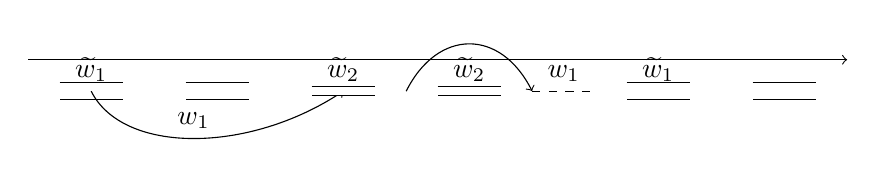
\begin{tikzpicture}[scale=0.8]
    % Draw the convolutional blocks
    \draw[double distance=2mm] (-3,0) -- (-2,0) node[midway, above] {$\widetilde{w}_1$};
    \draw[double distance=2mm] (-1,0) -- (0,0);
    
    % Draw the skip connections
    \draw[->] (-2.5,0) .. controls (-2,-1) and (0,-1) .. (1.5,0) node[pos=0.5,above] {$w_1$};
    
    % Draw the layer with single convolution
    \draw[double distance=1mm] (1,0) -- (2,0) node[midway, above] {$\widetilde{w}_2$};
    \draw[double distance=1mm] (3,0) -- (4,0) node[midway, above] {$\widetilde{w}_2$};
    
    % Draw the transpose operation
    \draw[dashed] (4.5,0) -- (5.5,0) node[midway, above] {$w_1$};
    
    % Draw the skip connection from the previous layer
    \draw[->] (2.5,0) .. controls (3,1) and (4,1) .. (4.5,0);
    
    % Draw the final convolutional block
    \draw[double distance=2mm] (6,0) -- (7,0) node[midway, above] {$\widetilde{w}_1$};
    \draw[double distance=2mm] (8,0) -- (9,0);
    
    % Draw the top arc for the skip connection
    \draw[->] (-3.5,0.5) to [out=0,in=180] (9.5,0.5);
\end{tikzpicture}

\end{document}